\documentclass{article}
\usepackage[margin=3cm]{geometry}
\usepackage{textcomp}
\usepackage{graphicx}
\usepackage{float}
\usepackage{amsmath}
\usepackage[hidelinks]{hyperref}
\urlstyle{same}

\newcommand{\suppfignorm}{1}
\newcommand{\suppfigtotals}{2}
\newcommand{\suppfigorder}{3}
\newcommand{\suppfigbiophys}{4}

\title{When normalization gets prickly: are spike-ins good enough for single-cell RNA sequencing data?}
\author{Aaron Lun, Fernando Calero, Liora Vilmovsky, Bertie G\"ottgens, John Marioni}

\begin{document}

\maketitle

\section{Introduction}
Single-cell RNA sequencing (scRNA-seq) is a powerful technique for studying transcriptional activity in individual cells.
Briefly, RNA is isolated from single cells, reverse transcribed into cDNA and sequenced using massively parallel sequencing technologies \cite{shapiro2013singlecell}.
This can be done on microfluidics platforms like the Fluidigm C1 \cite{pollen2014lowcoverage}, or with protocols such as Smart-seq2 \cite{picelli2014full} that use microtiter plates.
Gene expression is quantified by mapping the read sequences to the genome and counting the number of reads mapped to each gene.
To avoid amplification biases, individual transcript molecules can also be tagged with unique molecular identifiers (UMIs) \cite{islam2014quantitative}, such that sequencing to saturation and counting UMIs will yield the number of transcripts of each gene in a cell.
Regardless of whether reads or UMIs are used, not all transcript molecules will be captured and sequenced due to cell-specific inefficiencies in reverse transcription \cite{stegle2015computational}.
The presence of these cell-specific biases compromises the direct use of the read/UMI count as a quantitative measure of gene expression.
Normalization is required to remove these biases before counts can be meaningfully compared between cells.

A common normalization strategy for RNA-seq data uses a set of genes that have constant expression across cells.
This set can consist of pre-defined ``house-keeping'' genes, or it can be empirically defined under the assumption that most genes are not differentially expressed (DE) between cells \cite{lun2016pooling,anders2010differential,robinson2010tmm}.
Counts are scaled to eliminate differences in the coverage of this non-DE set across cells.
Here, the assumption is that these differences between cells must be technical in origin, e.g., due to differences in library size or composition bias \cite{robinson2010tmm}.
Downstream analyses are then applied to the scaled counts to avoid obtaining misleading results.
This gene-based approach works well for bulk sequencing experiments where the population-wide gene expression profile is stable.
However, it may not be suitable for single-cell experiments where the presence of strong biological heterogeneity complicates the identification of a reliable non-DE set. 
For example, house-keeping genes may be turned on or off by transcriptional bursting, while cell cycling and other processes may trigger large-scale changes in the transcriptional programme that preclude the assumption of a non-DE majority.

An alternative normalization strategy uses spike-in RNA for which the identity and quantity of all transcripts is known \cite{stegle2015computational}.
The same amount of spike-in RNA is added to each cell, and the spike-in transcripts are processed along with their endogenous counterparts into a sequencing library.
This yields a set of read (or UMI) counts for both endogenous and spike-in transcripts in each cell.
Normalization is performed by scaling the counts for each cell such that the counts for the spike-in genes are, on average, the same between cells.
The central assumptions of this approach are that (i) the same amount of spike-in RNA is added to each cell, and (ii) the spike-in and endogenous transcripts are similarly affected by cell-to-cell fluctuations in capture efficiency.
Under these assumptions, any differences in the coverage of the spike-in transcripts between cells must be artifactual in origin and should be removed by scaling.
One particular advantage of this strategy is that it does not make any assumptions about the endogenous expression profile, unlike the non-DE approach described above.
This means that spike-in normalization can be applied in situations where large-scale changes in expression (e.g., related to changes in total RNA content) are expected and of interest \cite{lun2016stepbystep}.

However, there are several criticisms of spike-in normalization that challenge the validity of its central assumptions.
The first is that the same quantity of spike-in RNA may not be consistently added to each sample \cite{robinson2010tmm}, while the second is that synthetic spike-in transcripts may not behave in the same manner as endogenous transcripts \cite{grun2015design}.
Any differences in spike-in quantity or behaviour across cells will compromise the accuracy of spike-in normalization \cite{risso2014normalization}.
This would complicate the analysis of data sets where a non-DE majority cannot be assumed -- if spike-in normalization cannot be used, there is no obvious alternative for removing cell-specific biases.
However, whether or not the aforementioned criticisms are valid in real scRNA-seq experiments is yet to be determined.

In this paper, we conduct a series of experiments to estimate the reliability of spike-in normalization in single-cell transcriptome studies employing plate-based protocols.
We use mixtures of two distinct spike-in RNA sets to quantify the variance of the added spike-in volume across cells.
We also estimate the variability in differential behaviour between the sets, to determine how cell-specific biases change between different RNA populations.
Both factors are quantitatively negligible and have only minor effects on the results of downstream analyses such as detection of DE and highly variable genes.
These results suggest that spike-ins can be safely used for routine normalization of scRNA-seq data.

% The advantage of spike-ins is that it can capture cell size and doesn't require a non-DE majority.
% However, is the cell size interesting, or should it be normalized out (in which case accurate spike-in addition wouldn't be required at all)?
% It's most obviously useful for cell cycle considerations -- possibly also cancer and in some aspects of differentiation.
% The Islam non-UMI dataset is one example where there seems to be a 20-50-fold increase in counts in the MEFs vs mESCs.
% 
% I guess spike-in normalization is more technically correct, even if you end up getting every gene as being DE (technically true in terms of molecules, but possibly irrelevant).
% Rankings definitely change - spike-in normalization would favour genes that are upregulated on top of an increase in RNA content (as these would be hugely significant).
% Standard normalization would have no preference as you seek the balance between the two extremes.
% On the other hand, any non-DE genes with no change in the molecule number will be called as significant in standard normalization, which is definitively wrong.
% You could have your cake and eat it by separating the DE list into up/down changes for easier examination of the up/down changes.

\section{Results}

\newcommand\variance{\mbox{var}}

\subsection{Overview of the mixture experiments}
We aimed to assess the variability in the added spike-in quantity across cells.
To do so, we performed mixture experiments using two distinct spike-in sets (Figure~\ref{fig:expdesign}) -- the External RNA Controls Consortium (ERCC) set and the Spike-in RNA Variants (SIRV) set.
An equal volume of each spike-in set was added separately to a single well of a 96-well microtiter plate.
Each well also contained a single mouse cell (416B cells or trophoblasts) to mimic real experimental conditions.
The resulting pool of endogenous/spike-in RNA in each well was used to generate a library with the Smart-seq2 protocol.
This process was repeated for multiple wells and sequencing was performed on all libraries.

\begin{figure}[tbp]
\begin{center}
\includegraphics[width=0.8\textwidth]{pics/plate_setup.pdf}
\end{center}
\caption{Schematic of the experimental design to assess the variability of spike-in addition in a plate-based scRNA-seq protocol.
(a) A cell is sorted into each well of a plate and lysed.
For one set of wells, an equal volume of each spike-in set is added separately, along with the reverse transcription (RT) reagents.
For another set of wells, an equal volume of a pooled mixture of the two spike-ins is added into each well (done twice to keep the protocol consistent).
Reverse transcription, PCR amplification, library generation and sequencing were then performed.
(b) The log$_2$-ratio between the total counts of the two spike-in sets was computed for each well.
The variance of the log-ratio was estimated from all wells with separate addition of spike-ins, and from wells with addition of the premixed pool.
The difference between these two estimates represents the variance attributable to volume addition.
}
\label{fig:expdesign}
\end{figure}

For each library, reads were mapped to the genome and assigned to genes to quantify expression.
The total count was computed across all transcripts of each spike-in set in each well.
The log$_2$-ratio of the totals between the two sets was computed for each well, and the variance of this log-ratio was computed \textit{across} wells.
Any variability in spike-in volume addition should manifest as an increase to the variability of the log-ratio, given that the spike-in sets were added independently to each well.

We also repeated the experiment by adding volumes of ``premixed'' spike-in solution where the two spike-in sets had been pooled at a 1:1 ratio.
This ensures that there is no well-to-well variability in the relative quantities of RNA from the two spike-in sets.
The variance of the log-ratio across these premixed-addition wells provides a baseline level of variability in the protocol (e.g., due to sequencing noise).
The variance of volume addition was then estimated as the difference in the variance estimates from the premixed-addition wells and from the wells with separate addition of spike-ins.

We performed both the premixed and separate-addition experiments on the same plate to avoid plate effects \cite{hicks2015widespread,tung2016}.
For the separate-addition experiment, we also reversed the order of addition of the two spike-in sets to determine if this affected the variance estimate.
Finally, we generated data from replicate plates to ensure our results were reproducible.
This was done in a range of conditions, i.e., using different cells, by different operators and with sequencing by different machines and centres.

We used a protocol based on microtiter plates rather than microfluidics as it is easier to customise the spike-in addition step in the former.
Our experimental design requires two separate additions of spike-in RNA to each reaction (see Methods).
This is not straightforward to achieve on, say, the Fluidigm C1 chip where the added volume for each reagent depends on the design on the reaction chamber.
Plate-based protocols also tend to be cheaper and are compatible with existing laboratory techniques such as indexed fluorescently-activated cell sorting (FACS).
Thus, we focus on normalization of data from plate-based protocols, to reflect their increasing use in single-cell studies (CITE).

\subsection{Estimating the variance of volume addition}
Denote the log$_2$-transformed total count for well $i$ and spike-in set $s$ as
\[
T_{is} = \log_2 \left[ L_i l_s V_{is} R_{is} \sum_{t_s} r_{t_s} c_{t_s} \right] + \varepsilon_{is}
\]
where $c_{t_s}$ is a constant specifying the concentration (in terms of transcripts per unit of volume) of each spike-in transcript $t_s$;
$r_{t_s}$ is a constant specifying the optimal transcript molecule-to-cDNA fragment capture rate for $t_s$;
$R_{is}$ is a random variable representing the average capture efficiency in well $i$ for all transcripts in set $s$;
$V_{is}$ is a random variable representing the volume of solution of $s$ added to $i$;
$L_i$ is a random variable representing the cDNA fragment-to-read conversion rate for $i$, scaled by a constant $l_s$ representing the ``sequenceability'' of transcripts in $s$;
and $\varepsilon_{is}$ is the error term attributable to sequencing noise and variability in library preparation, where $E(\varepsilon_{is})=0$ and $\variance(\varepsilon_{is})= \sigma^2_{lib(s)}$.
We assume that $R_{is}$, $V_{is}$ and $\varepsilon_{is}$ are mutually independent of each other, as they relate to separate steps in the protocol.
We also assume that $V_{is}$ and $\varepsilon_{is}$ are independent between different $s$ (but not $R_{is}$, due to well-specific factors affecting capture efficiency for all transcripts).
Further details on the interpretation of these variables are provided in Section~BBB of the Supplementary Materials.

Let $s=1$ represent the ERCC spike-in set and $s=2$ represent the SIRV spike-in set.
In the experiment where each spike-in set is added separately to each well, denote the log$_2$-ratio of the total counts between the two sets as $\theta_i = T_{i1} - T_{i2}$ for well $i$.
This can also be written as
\[
\theta_i = \log_2(V_{i1}) + \varepsilon_{i1} - \log_2(V_{i2}) - \varepsilon_{i2} + F_i
\]
where $F_i = \log_2(R_{i1}/R_{i2})$ and represents the log-fold change in the average capture efficiency between the two sets (i.e., the difference in behaviour of the transcripts).
Computing the variance of $\theta_i$ yields
\[
\variance(\theta_i) = 2 \sigma^2_{vol} + \sigma^2_{lib(1)} + \sigma^2_{lib(2)} + \variance(F_i)
\]
where $\sigma^2_{vol}$ is the variance of $\log_2 V_{i1}$ and $\log_2 V_{i2}$.
The volume addition procedure is the same for each spike-in set, so $V_{i1}$ and $V_{i2}$ should have the same distribution.
Also, we consider the variance of $F_i$ because $R_{i1}$ and $R_{i2}$ are not independent, e.g., due to well-specific effects on capture efficiency.

In the experiment where the spike-in sets are premixed before addition, $V_{i1}=aV_{i2}$ for some constant $a$ representing the proportions in which the two sets are mixed.
(This should be close to unity.)
If the same premixed solution is added to each well, the relative volume of ERCC spike-ins to SIRV spike-ins must be constant for all wells.
This means that the log$_2$-ratio for the premixed experiment is 
\[
\theta^*_i = \log_2(a) + \varepsilon_{i1} - \varepsilon_{i2} + F_i \;.
\]
As $a$ is constant for all $i$, the variance of $\theta^*_i$ is
\[
\variance(\theta^*_i) = \sigma^2_{lib(1)} + \sigma^2_{lib(2)} + \variance(F_i) \;.
\]
This represents the technical variance attributable to the rest of the scRNA-seq protocol.
To obtain an estimate of the variance of the volume addition step, simple arithmatic yields
\[
\sigma^2_{vol} = \frac{\variance(\theta_i) - \variance(\theta^*_i)}{2} \;.
\]
It should be stressed that this variance estimate is relevant to all experiments using the same protocol for spike-in addition, even if the identity or concentration of the spike-in set is different.

Using this mathematical framework, we proceeded to estimate the variance components from the data from our mixture experiments.
We observed that the log-ratios $\theta_i$ and $\theta^*_i$ computed from each plate were roughly normally distributed (Supplementary Figure~\suppfignorm{}).
Thus, we fitted a linear model to each set of log-ratios and used the residual variance of the fit as our estimate of $\variance(\theta_i)$ or $\variance(\theta^*_i)$.
Linear models are particularly useful as they allow blocking on additional structure in the experimental design (Methods).
In addition, the size of $T_{is}$ was similar between wells with premixed or separate addition of spike-ins, which simplifies the calculation of $\sigma^2_{vol}$ (see Supplementary Figure~\suppfigtotals{}, Section~XX of the Supplementary Materials for more details).
Finally, the order of spike-in addition did not affect the variance estimates for the separate-addition wells on most plates (Supplementary Figure~\suppfigorder{}).

Our results indicate that $\sigma^2_{vol}$ is consistently smaller than the variance in the rest of the protocol (Figure~\ref{fig:varestimates}).
Indeed, no significant difference was detected between $\variance(\theta_i)$ and $\variance(\theta^*_i)$ for each plate.
This indicates that variability of spike-in volume addition is a minor contributor to the technical variability of the spike-in counts.
To further put these estimates into context, consider that $T_{is}$ represents the log$_2$-transformed ``size factor'' for the library generated from well $i$.
In other words, all counts in this library are scaled by a factor of $2^{-T_{is}}$ to correct for well/cell-specific biases during spike-in normalization.
The variance of the log-size factors is several orders of magnitude larger than $\sigma^2_{vol}$.
This suggests that the latter will not have a major effect on the normalization result.

\begin{figure}[btp]
    \begin{center}
        \includegraphics[height=2.2in,trim=0mm 10mm 0mm 10mm,clip]{../real/pics/variance_exp.pdf}
        \includegraphics[height=2.2in,trim=0mm 10mm 0mm 10mm,clip]{../real/pics/variance_sf.pdf}
    \end{center}
    \caption{Variance estimates of the log$_2$-ratio between the ERCC and SIRV total counts (left), or the log$_2$-size factors computed from those totals (right).
        Each estimate is the residual variance of a linear model fitted to the log-ratios or log-size factors across all cells (416B or trophoblasts) in each plate.
        Error bars represent the standard errors of the estimates, assuming normally-distributed values.
    }
    \label{fig:varestimates}
\end{figure}

\subsection{Estimating the variance of capture efficiency}
The variance of $F_i$ is also relevant as it determines the effect of differences in behaviour between distinct sets of transcripts.
Even when the capture efficiency differs between sets, spike-in normalization may still be appropriate \textit{provided that the fold change in capture efficiency is the same in all wells}.
Consider a situation where there is a consistent increase in efficiency in the spike-in set relative to endogenous transcripts.
This scales up the counts for the spike-in transcripts in all libraries by the same amount, which cancels out between libraries (i.e., the fold changes between counts for endogenous or spike-in transcripts in different libraries are unaffected).
However, if the fold change in efficiency varies across wells, the accuracy of spike-in normalization is compromised.
This is because changes in the capture efficiency for the spike-in transcripts are confounded with changes in efficiency for all transcripts in the well, precluding the use of spike-ins to normalize the counts for the endogenous trancripts.

In our mathematical framework, the estimated variance of $\theta^*_i$ provides an upper bound for the variance of $F_i$.
This quantifies the extent to which normalization is affected by differences in efficiency between two transcript sets.
We observe that $\variance(\theta^*_i)$ is an order of magnitude lower than the variance of the log-size factors in each plate (Figure~\ref{fig:varestimates}).
This indicates that the variance in efficiency across wells, while greater than $\sigma^2_{vol}$, is still relatively small compared to the other factors driving normalization, e.g., differences in cellular RNA content, well-to-well variability in capture efficiency for all transcripts.
Obviously, $F_i$ is computed between two spike-in sets whereas the differences between synthetic spike-in and endogenous transcripts are likely to be greater.
Nonetheless, the SIRV and ERCC spike-ins do vary in their biophysical properties (Supplementary Figure~\suppfigbiophys{}).
For example, the SIRV transcripts have more variable length and lower GC content compared to the ERCC transcripts.
This suggests that $F_i$ will include some of the differences in behaviour between synthetic and endogenous RNA, such that $\variance(F_i)$ can be used as a rough estimate of the magnitude of the associated variability.

\subsection{Assessing the downstream effect of variability with simulations}
We assessed whether the results of downstream analyses using spike-in normalization were sensitive to variability in spike-in addition or behaviour.
First, we obtained data from plate-based experiments that contained counts for spike-in transcripts.
This included public data sets \cite{someone,islam2011characterisation,wilson2015combined} as well as our 416B and trophoblast data.
We then performed analyses such as detection of differentially expressed genes (DEGs) and highly variable genes (HVGs), as well as dimensionality reduction and clustering of cells.
This was done without any modification of the data, yielding a set of original results.

Next, we designed simulations based on each of the real data sets (see Methods).
Briefly, the total spike-in count for each well was scaled by a randomly sampled factor $2^X_i$, where $\variance(X_i)$ was set to our experimental estimate of spike-in variance.
Counts for the individual spike-in transcipts were rescaled to reflect this new total.
Analyses were performed on the simulated data and compared to the original results.
Any changes indicate that the analysis is sensitive to spike-in variability in real experiments.
The advantage of this approach is that only the spike-in counts are modified.
Counts for endogenous genes were used directly without modification, ensuring that the simulations are realistic.

For DEG detection, we applied edgeR \cite{robinson2010edgeR} and MAST \cite{finak2014mast} to the original and simulated data after spike-in normalization.
We observed only minor (below 5\%) changes to the set of significant DEGs from either method upon introducing spike-in variability in each data set (Figure~\ref{fig:setchange}a). 
Small changes were also observed in the top 200 DEGs with the smallest $p$-values.
For HVG detection, we applied methods based on the coefficient of variation \cite{brennecke2014technical} or on the variance of log-expression values \cite{lun2016step}.
Again, only minor changes were observed in most data sets (Figure~\ref{fig:setchange}b), for both the set of significant HVGs and for the top 200 HVGs with the smallest $p$-values.
These results suggest that the detection and ranking of DEGs and HVGs are largely robust to variability in spike-in volume or behaviour.

\begin{figure}[bt]
    \begin{center}
        \includegraphics[height=2.5in,trim=0mm 5mm 0mm 10mm,clip]{../simulations/pics/de_plot.pdf}
        \includegraphics[height=2.5in,trim=0mm 5mm 0mm 10mm,clip]{../simulations/pics/hvg_plot.pdf}
    \end{center}
    \caption{Effect of spike-in variability on DEG or HVG detection in simulated data.
        Left: The percentage change in the set of DEGs detected in each data set at a FDR of 5\% by edgeR or MAST.
        This was also calculated for the top set of 200 DEGs with the smallest $p$-values.
        Simulations were designed to test for differential expression between mouse embryonic stem cells (mESCs) and fibroblasts (MEFs) \cite{islam2011characterisation},
        or before and after induction of the CBFB-MYH11 oncogene in our 416B data set.
        Right: The percentage change in the set of HVGs detected in each data set at a FDR of 5\%,
        by the Brennecke \textit{et al.} method using the squared coefficient of variation (CV$^2$) or by the variance of log-expression.
        This was also calculated for the top set of 200 HVGs with the smallest $p$-values.
        Simulations were designed to detect HVGs in our 416B and trophoblast data, and in haematopoietic stem cells (HSCs) \cite{wilson2015combined}.
        All values represent the mean of 20 simulation iterations, and error bars represent standard errors.
    }
    \label{fig:setchange}
\end{figure}

For dimensionality reduction, we restricted ourselves to principal components analysis (PCA) on the normalized expression profiles of all cells. 
While $t$-distributed stochastic neighbour embedding \cite{vanhinton2008tsne} is commonly used, its robustness is difficult to evaluate due to its randomness.
We generated PCA plots of the first three principal components using both the original and simulated data.
At each simulation iteration, coordinates of all cells in the simulated plots were mapped onto the corresponding original plots to determine the sensitivity of the original locations to spike-in variability.
Figure~\ref{fig:dimclust}a indicates that changes in the location of each cell across simulation iterations were generally minor.
Thus, spike-in variability does not appear to affect the visual interpretation of PCA plots.

\begin{figure}[btp]
    \begin{center}
        \includegraphics[width=\textwidth]{../simulations/clustering/pca_effect.pdf}
        \includegraphics[width=\textwidth]{../simulations/clustering/clusters.pdf}
    \end{center}
    \caption{Effect of spike-in variability on dimensionality reduction and clustering in simulated data.
        (a) PCA plots of the first three principal components, where each cell is coloured according to the annotated cell type in the original study \cite{someone}.
        The circle around each cell contains 95\% of remapped locations across the simulation iterations, and represents the deviation due to spike-in variability.
        (b) Clusters were identified from the original data by hierarchical clustering with Ward's criterion, followed by a tree cut with $k$ of 2, 5 or 10.
        This was repeated at each simulation iteration, and the maximum Jaccard index of each original cluster to any of the simulated clusters at the same $k$ was computed.
        Each value represents the mean of 20 simulation iterations, and the error bars represent standard errors.
        (c) The maximum Jaccard index for each original cluster generated with Ward's criterion, when compared to the clusters generated from complete-linkage clustering of the original data.
    }
    \label{fig:dimclust}
\end{figure}

Finally, we performed hierarchical clustering and applied a tree cut to identify clusters of cells in the original data.
This was repeated at each simulation iteration to obtain a corresponding set of simulated clusters.
For each original cluster, we computed the Jaccard index with respect to each of the simulated clusters, and we recorded the maximum value across all simulated clusters.
A large maximum Jaccard index means that the original cluster is successfully recovered in one of the simulated clusters.
We observed that the maximum Jaccard indices were moderate to large (Figure~\ref{fig:dimclust}b), with values above 0.6 for most of the original clusters.
To put this into context, we repeated the clustering on the original data but using a different algorithm.
This yielded smaller indices for all clusters (Figure~\ref{fig:dimclust}c), indicating that spike-in variability has less effect on the results than the choice of clustering method.

\section{Discussion}

\section{Methods}

\subsection{Spike-in mixture experiments with Smart-seq2}
% On a single plate, so no plate effects.
% Mention cutting up of plate, especially for the two conditions.
% No effect of different cell treatments.

\subsection{Data analysis for the mixture experiments}
Reads were mapped to the mm10 build of the mouse genome, including sequences of transcripts in the ERCC (\url{https://tools.thermofisher.com/content/sfs/manuals/ERCC92.zip}) and SIRV (\url{https://www.lexogen.com/wp-content/uploads/2015/11/SIRV_Sequences_151124.zip}) spike-in sets.
Mapping was performed using the subread aligner v1.5.0 \cite{liao2013subread} in single-end RNA-seq mode with unique alignment.
Reads with mapping qualities greater than or equal to 10 were counted into exonic regions of genes using the featureCounts function in the Rsubread package v1.20.1 \cite{liao2014featurecounts}.
Genes were defined using Ensembl v82 annotation for the GRCm38 mouse assembly and annotation for the ERCC and SIRV transcripts.
This yielded a count for each endogenous gene and spike-in transcript in each well.

Variance components were estimated from the libraries generated from a single plate.
In each well, the sum of counts across all transcripts in each spike-in set was computed, and the log$_2$-ratio between the ERCC and SIRV sums was calculated.
To estimate $\variance(\theta_i)$, a linear model with a one-way layout was fitted to the log-ratios for all wells where the two spike-in sets were added separately.
In each plate of the 416B data set, each combination of treatment (control or oncogene-induced) and spike-in addition order (ERCC or SIRV first) was treated as a group in the one-way layout.
In each plate of the trophoblast data, only the spike-in addition order was used to define the groups.
After fitting the model, the mean of the squared residual effects was used as an estimate of $\variance(\theta_i)$.
This was repeated for $\variance(\theta^*_i)$ using all wells where premixed spike-ins were added.
Here, addition order was irrelevant so the one-way layout contained only the two treatment groups in the 416B data set.
Similarly, only a single group was defined for the trophoblast data.
Linear modelling ensures that any changes in the mean log-ratio across groups do not inflate the variance estimate.
Note that we fit linear models to each plate separately, to check whether the estimates are consistent across replicate plates.

To detect differences in the variance estimates for premixed and separate addition, an F-test for the equality of variances was applied.
Significant differences were defined by rejecting the null hypothesis at a type I error rate of 5\%.
We calculated $\sigma^2_{vol}$ from estimates of $\variance(\theta_i)$ and $\variance(\theta^2_i)$, using the expression described above.
However, if the difference between $\variance(\theta_i)$ and $\variance(\theta^2_i)$ was negative, $\sigma^2_{vol}$ was set to zero instead.
To assess the effect of the order of spike-in addition, a linear model was fitted to the subset of relevant wells on each plate to obtain an order-specific variance estimate.

\subsection{Simulation design for resampling spike-in variability}
For each data set, we compute $T_{is}$ for each cell $i$ and spike-in set $s$.
The variance of $T_{is}$ is
\[
    \variance(T_{is}) \approx \sigma^2_{lib(s)} + \sigma^2_{vol} + \variance(R_{is}) + \variance(\log_2 L_i)
\]
where the approximation assumes that $L_i$ is independent of the other random variables.
This is generally reasonable as $L_i$ is mainly determined by factors not related to spike-in volume or behaviour, such the number of cDNA fragments derived from endogenous transcripts.
Let $R_{is} = R_{i0}P_{is}$, where $R_{i0}$ is the well-specific average capture efficiency of endogenous transcripts and $P_{is}$ is the fold change in average efficiency of the transcripts in $s$ over their endogenous counterparts.
We assume that $R_{i0}$ and $P_{is}$ are independent for each well, and that $\log_2(P_{is})$ can be approximated with $F_i$ (i.e., the log-fold change in average efficiency between SIRV and ERCC spike-ins).
This yields
\[
    \variance(T_{is}) \approx \sigma^2_{lib(s)} + \sigma^2_{vol} + \variance(F_i) + \variance(R_{i0}) + \variance(\log_2 L_i) \;.
\]

% If library quantification has been performed, then L_i will be more likely to be correlated with volume because everything competes against each other.
% At least it won't be correlated with global capture efficiency, as this should cancel out.
% If it hasn't been performed, then L_i should be constant so it shouldn't matter.
% The independence assumption means that we do not have to rescale the cellular counts to reflect variable undersampling.
% Doing so would be problematic, as direct scaling of the counts would distort the empirical mean-variance relationship of the count data.

Let us denote $x^2 = \sigma^2_{vol} + \variance(F_i)$, representing the total variance attributable to spike-in addition and capture efficiency.
We also denote $\hat\sigma^2_s$ as the estimate of $\variance(T_{is})$ across wells, and $\hat\mu_s$ as the estimate of $E(T_{is})$.
We use $\variance(\theta^*_i) \approx 0.01$ as our estimate $\hat{x}^2$ of the upper bound of $x^2$, following the reasoning described previously.
For each well $i$, we compute a simulated log$_2$-total $T^*_{is}$ as
\[
    T^*_{is} = (T_{is} - \hat\mu_s)\sqrt{1-\frac{ \hat{x}^2}{\hat\sigma^2_s}} + \hat\mu_s + X_i
\]
where $X_i \sim \mbox{Normal}(0, \hat{x}^2)$ and is independently sampled for each well.
This approach ensures that $\variance(T^*_{is}) = \hat\sigma^2_s$.
In contrast, if $X_i$ were directly added to $T_{is}$, the variance of $T^*_{is}$ would be inflated as $x^2$ is already present in $\variance(T_{is})$, i.e., the contribution of spike-in variance would effectively be doubled.

Counts for the library generated from each well were rescaled to reflect the new, simulated log-total.
A quantile adjustment approach was used to preserve the empirical mean-variance relationship.
Briefly, a negative binomial generalized linear model (NB GLM) was fitted to the counts across all wells for each spike-in transcript, using the mglmOneGroup function in edgeR \cite{mccarthy2012differential, robinson2010edgeR} with an all-intercept design matrix and $T_{is}$ (converted to base $e$) as the offset for well $i$.
An abundance-dependent trend was also fitted to the NB dispersions across all spike-in transcripts using the estimateDisp function.
For each transcript $t$, we assumed that the count $y_{ti}$ for well $i$ was sampled from a NB distribution with mean equal to the corresponding fitted value of the GLM and dispersion equal to the fitted value of the mean-dispersion trend.
We scaled the NB mean by $2^{T^*_{is} - T_{is}}$ to obtain a modified NB distribution.
We identified the tail probabilities of $y_{ti}$ in the original distribution, and identified the corresponding quantile with the same tail probabilities in the modified distribution, using the q2qnbinom function \cite{robinson2008small}.
This new quantile was used as the simulated count for the corresponding gene and cell.

% The estimation of the true parameters conditions on the observed spike-in totals, and doesn't make the assumption that spike-in totals are constant.
% For example, if it turned out that you added half the amount of spike-in to one well, it wouldn't distort the estimation of the (conditional) mean.
% Okay, maybe the trended dispersion would be a bit weird, because technical variability should depend on the amount of RNA, but some inaccuracy there is forgivable.

\subsection{Evaluating the robustness of DEG detection}
Two data sets were used to test the effect of spike-in variability on DEG detection.
The first was the 416B data generated previously, where DEGs were detected between control and oncogene-induced cells in both plates.
Here, we used an additive model with a treatment term and a blocking factor for the plate.
The second data set was obtained from the NCBI Gene Expression Omnibus (GEO) under the accession number GSE29087, and compared mouse embryonic stem cells and fibroblasts \cite{islam2011characterization}.

In both studies, DEGs were detected between conditions using edgeR \cite{robinson2010edgeR} and MAST \cite{finak2015mast}.
The former represents methods designed for analyses of bulk RNA-seq data, while the latter represents specialized single-cell methods.
For each method, spike-in normalization was performed by scaling the counts such that the spike-in totals were the same between cells.
The set of DE genes in the original data was then identified at a FDR of 5\% (see Section~Y in the Supplementary Materials for implementation details of each method).
This was repeated for the simulated data, and the proportion of DEGs common to both the original and simulated sets was computed.
The common proportion of the top 200 genes with the smallest $p$-values was also computed.
This was repeated for 20 simulation iterations, and the average proportion across iterations was reported for each method.

\subsection{Evaluating the robustness of HVG detection}
Three data sets were used to test the effect of spike-in variability on HVG detection.
This included the 416B and trophoblast data sets generated previously.
In the former, blocking was performed to remove plate- and treatment-specific effects on mean expression, i.e., HVGs were detected within treatment conditions on each plate.
Similarly, blocking was performed on the plate of origin for each cell in the trophoblast data set to remove plate effects.
The final data set was obtained from NCBI GEO under the accession number GSE61533 and contained a single plate of haematopoietic stem cells \cite{wilson2016 combined}.

In each data set, spike-in normalization was performed and HVGs were detected using two approaches based on spike-ins (see Section~Y in the Supplementary Materials for implementation details of each method).
The first approach is based on the method of Brennecke \textit{et al.} \cite{brennecke2013accounting} where the squared coefficient of variation for each gene is tested for a significant increase above technical noise.
The second approach is based on the variance of the log-normalized expression values \cite{lun2016step}, which provides some more robustness against outlier expression patterns.
Each method was applied on the original and simulated data, and a set of significant HVGs was detected at a FDR of 5\%.
The proportion of HVGs common to both the original and simulated sets was computed, along with the common proportion among the top 200 genes with the lowest $p$-values.
This was repeated for 20 simulation iterations, and the average proportion across iterations was reported for each method.

\subsection{Evaluating dimensionality reduction and clustering}
Count data from a study of pancreatic islet cells \cite{someone} was obtained from ArrayExpress under the acession E-MTAB-5061.
Spike-in normalization was performed and a set of HVGs was defined using the variance-of-log-expression method.
PCA plots of the first three components were constructed from the matrix of log-expression values for the HVGs.
This process -- including HVG detection -- was repeated with the simulated data after introducing spike-in variability.
To compare each simulated PCA plot to the original plot, the coordinates of each cell in the former were mapped onto the latter by rescaling and rotation.
Robustness was assessed based on the spread of remapped coordinates from all simulation iterations for each cell.
See Section~Y in the Supplementary Materials for details.

To test the robustness of clustering, the matrix of Euclidean distances between cells was computed from the HVG log-expression values. 
Hierarchical clustering was performed using the Ward criterion and the resulting dendrogram was cut into 2, 5 or 10 clusters.
(This was done using the hclust and cutree commands, respectively, from the stats package.)
This process was repeated with the simulated data, and the Jaccard index between every pair of simulated and original clusters was computed.
For each original cluster, the maximum Jaccard index across all simulated clusters was recorded at each simulation iteration.
This value represents the extent to which the membership of the original cluster was preserved in the most similar simulated cluster.
We also compared the original clusters to those generated from complete-linkage clustering of the original HVG log-expression values.

{\small
\bibliography{refnorm}
\bibliographystyle{unsrt}
}

\end{document}
